\documentclass{article}
\usepackage{ctex}
\usepackage{geometry}
\geometry{top = 2cm, left = 1cm, right = 1cm, bottom = 2cm}
\usepackage{amsmath,amssymb,amsthm,amsfonts}
\usepackage{abstract}
\usepackage{siunitx}
\usepackage{graphicx}
\usepackage{booktabs}
\usepackage{appendix}
\usepackage{hyperref}

\renewcommand{\appendixpagename}{附录}


\title{高纯锗(HPGe)$\gamma$射线谱仪}
\author{钱思天 2001112187}
\begin{document}
    \maketitle
    \begin{abstract}
        本实验利用了高纯锗(HPGe)谱仪探测器,对$^{60}\text{Co},^{152}\text{Eu}$源、环境本底以及矿渣样本进行测量。
        通过对$^{152}\text{Eu}$源的测量,对探测系统进行了相对效率刻度,而后,通过对$^{60}\text{Co}$源的测量,对实验测量系统做了绝对效率刻度。而后,通过调节放大倍数并重新刻度,让探测器能够探测矿渣中的$\gamma$射线,进而判断出矿渣中所含有的元素。
        \newline
        \newline
        {\emph{ 关键词:\ 高纯锗$\gamma$射线谱仪、探测效率刻度、未知成分探测 }\rm}

    \end{abstract}

    \section{背景简介}
    \subsection{高纯锗$\gamma$射线谱仪}
    $\gamma$射线是原子核衰变或裂变时放出的辐射,本质上它是一种能量比可见光和$X$射线高得
多的电磁辐射。利用$\gamma$射线与物质相互作用的规律,人们已设计出多种类型的$\gamma$射线的探测
器。用于测量$\gamma$射线能量和强度的仪器称为$\gamma$能谱仪,谱仪一般有射线探测器和电子学系统
两大部分。最常用的有 NaI(Tl)闪烁谱仪和高纯锗(HPGe)半导体谱仪。闪烁探测器是利用某些
物质在射线作用下发光的特性来探测射线的仪器。HPGe 探测器是利用$\gamma$光子与探测介质原
子发生相互作用产生次级电子,通过次级电子在介质中的电离效应来探测射线的仪器。本实
验介绍一种高分辨率的高纯锗$\gamma$谱仪。
高纯锗探测器(High-Purity Germanium 简称 HPGe 探测器)实质上是利用纯度极高的锗制
成的 P-N 探测器。由于锗的纯度极高,也就是杂质浓度很低,因而电阻率很大,可得到较厚
的耗尽层,又由于锗的原子序数高,适合于探测$\gamma$射线。HPGe 探测器具有能量分辨率极高
的优点,所以它被广泛应用于$\gamma$射线能谱的测量,使$\gamma$谱学的面貌发生了根本的变化。
近年来,在核谱学、核反应、核工程和核技术应用等方面,HPGe 探测器已成为分析复
杂$\gamma$能谱的不可缺少的工具。
\subsection{实验目的}
\begin{enumerate}
    \item 了解高纯锗(HPGe)γ射线谱仪的原理、一般操作以及数据采集、处理的方法等;
    \item 利用$^{60}\text{Co}$,$^{152}\text{Eu}$做探测效率刻度;
    \item 测定未知样品的种类、活度。
\end{enumerate}
\section{实验介绍}
\subsection{实验装置}
本实验用到的实验装置比较简单,有:
\begin{enumerate}
    \item 高纯锗谱仪一套;
    \item NIM机箱、插件式高压电源、低压电源、主放大器各一个;
    \item 多道数据采集以及微机系统一套。
    \item $^{60}\text{Co},^{152}\text{Eu}$放射源各一个;
    \item 未知矿渣样品及固定装置一套。
\end{enumerate}
\subsection{实验操作}
鉴于上一位同学实验结束时的状况,实验步骤调整如下:
\begin{enumerate}
    \item 连接电子学线路,
检查无误后给高纯锗探头加高压至$3500\si{V}$。并且沿用上一位同学成功的放大倍数$(50\times1.12)$。
    \item 测定环境本底与矿渣样品能谱,各20分钟。
    \item 测量$^{152}\text{Eu}$十分钟,利用此数据及接下来测量的$^{60}\text{Co}$数据进行刻度。
    \item 将主放大器的放大倍数调至两倍$(100\times 1.12)$,而后分别测量$^{60}\text{Co},^{152}\text{Eu}$及环境本底各10分钟,并利用他们进行刻度。
\end{enumerate}
\section{数据处理}
\subsection{利用$^{60}\text{Co}$的测量结果,计算谱仪的相关性能参数}
$^{60}\text{Co}$的测量谱如图\ref{fig:60Co},根据测量结果,可以计算出谱仪的相关性能参数,如谱仪分辨率,峰康比和相对探测效率。
\begin{figure}[htbp]
    \centering
    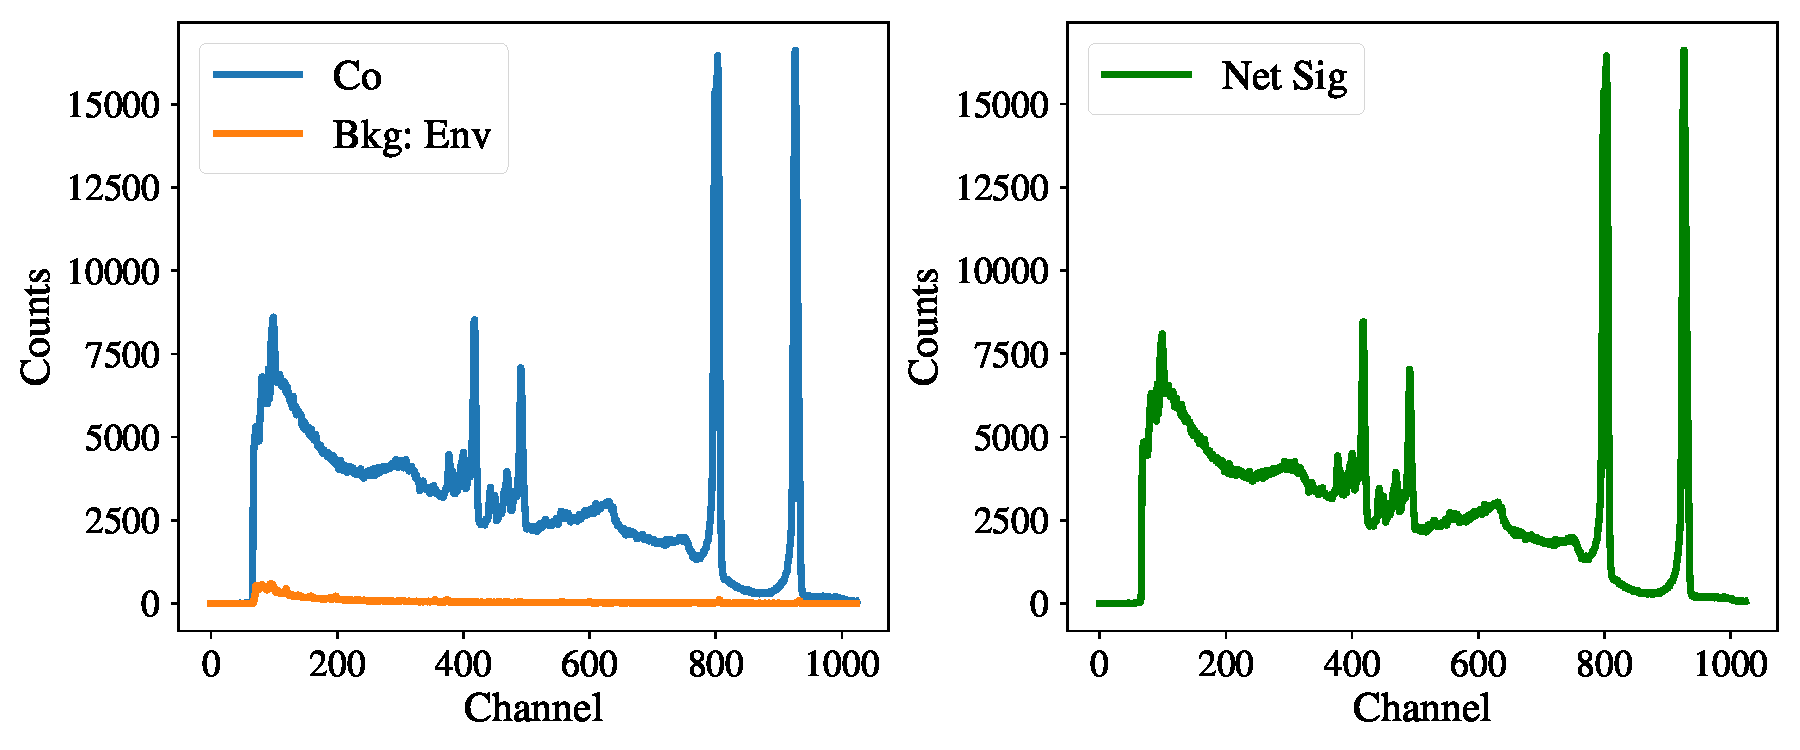
\includegraphics[width=\textwidth]{../plots/Co_net.pdf}
    \caption{$^{60}\text{Co}$放射源的测量结果\label{fig:60Co}}
\end{figure}
为了测算谱仪分辨率等,需要采用$^{60}\text{Co}$的两个特征峰,如图\ref{fig:60Co2Peak}。
\begin{figure}
    \centering
    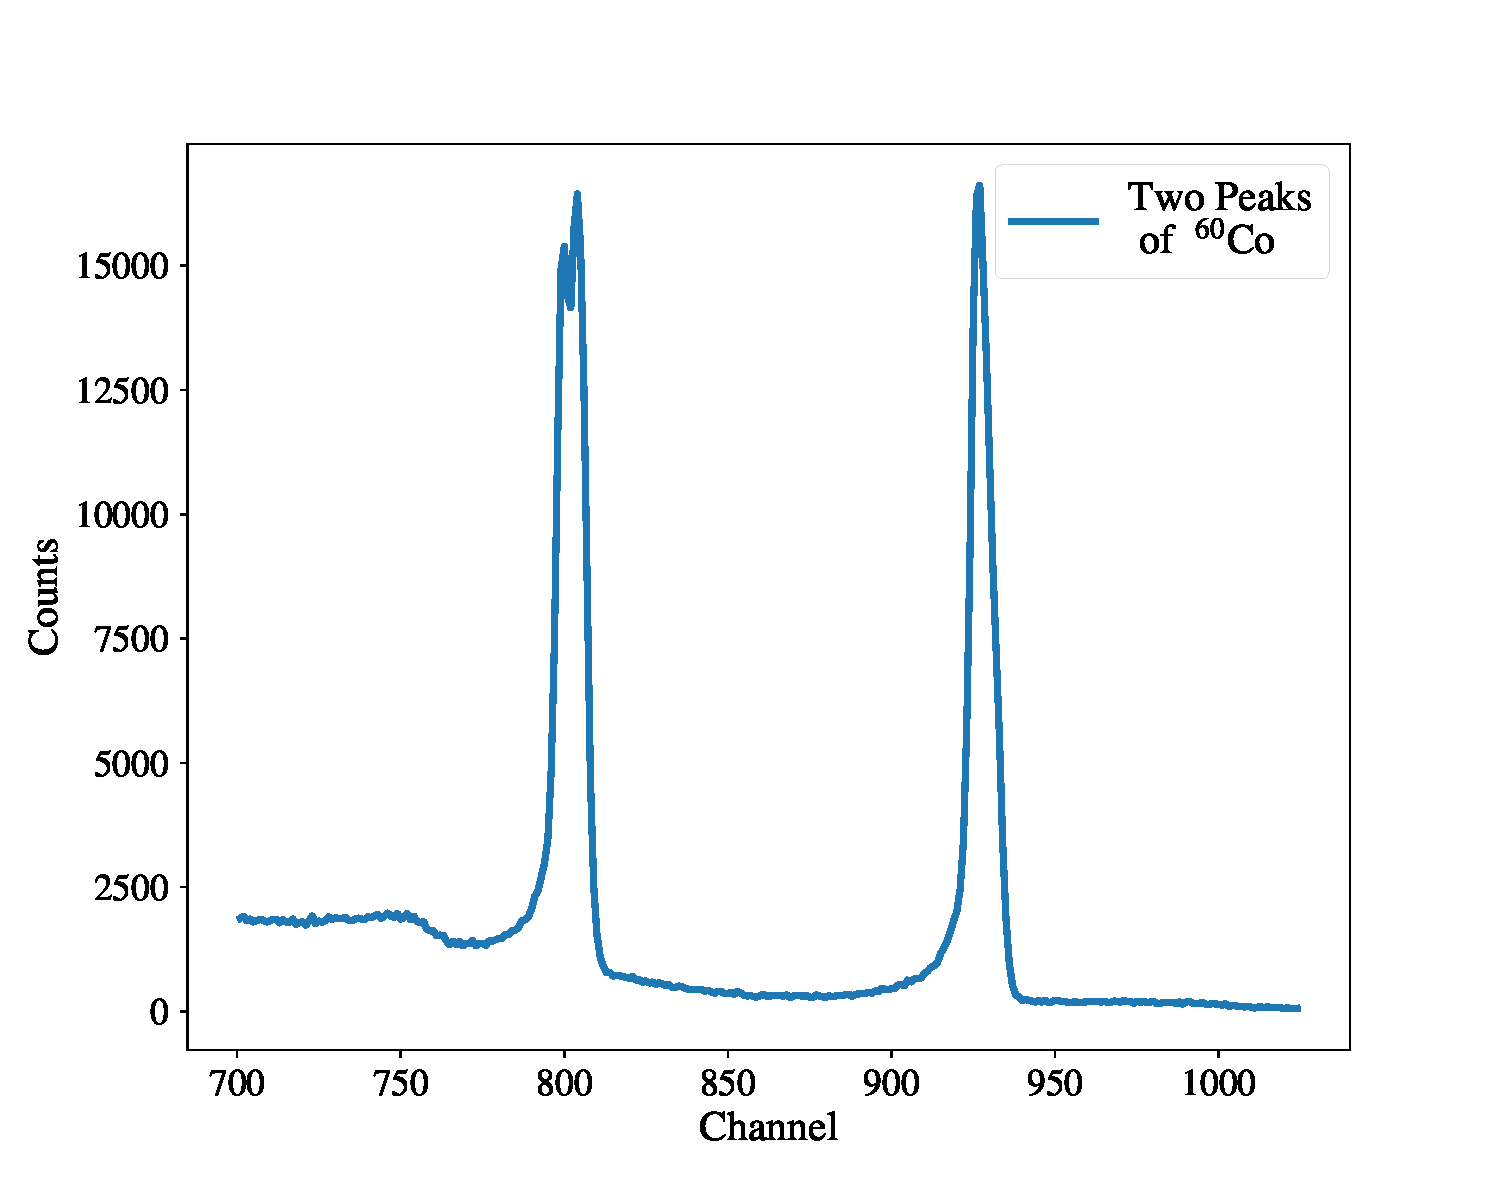
\includegraphics[width=0.6\textwidth]{../plots/Co_two_Peak.pdf}
    \caption{$^{60}\text{Co}$的两个特征峰\label{fig:60Co2Peak}}
\end{figure}
利用PHA18软件进行寻峰操作,可得结果如表\ref{tab:60Co},易知峰No.2为$1.33\si{MeV}$全能峰。其他的测量结果为
\begin{enumerate}
    \item 康普顿平台平均计数:4459.5;
    \item 活时$\si{528 s}$。
\end{enumerate}
\begin{table}[htbp]
    \centering
    \caption{$^{60}\text{Co}$的两个峰的测量结果\label{tab:60Co}}
    \begin{tabular}{lrrrr}
\toprule
Peak &  Channel &  FWHM &  Peak Counts &  Peak Area \\
\midrule
No.1    &      803 &   9.9 &        16472 &     193183 \\
No.2    &      926 &   7.7 &        16633 &     149863 \\
\bottomrule
\end{tabular}
\end{table}
计算可得:
\begin{enumerate}
    \item 谱仪的能量分辨
    \begin{equation}
        \text{FWHM}*\frac{1332.5-1173.2}{826-803} = 9.97\si{KeV}
    \end{equation}
\item 峰康比:3.73;
\item 相对探测效率:
\begin{equation}
    \varepsilon_{ref} = \frac{S}{Dt} = 0.3\%
\end{equation}
\end{enumerate}
\subsection{刻度}
原则上说,既然道址和能量存在线性正比关系,那么最少利用两个点就可以进行刻度。仅利用$^{60}\text{Co}$刻度的结果为:
\begin{equation}
    E = 1.2591*\text{Ch} + 133.22
\end{equation}
但是,仅仅利用$^{60}\text{Co}$能谱的两个峰进行刻度,结果难免会有测量误差导致的偏差。利用刻度结果对$^{152}\text{Eu}$进行刻度,可得因此,刻度选用$^{152}\text{Eu}$的各能量峰进行。对$^{152}\text{Eu}$的测量结果如图\ref{fig:152Eu_Full}所示:
\begin{figure}[htbp]
    \centering
    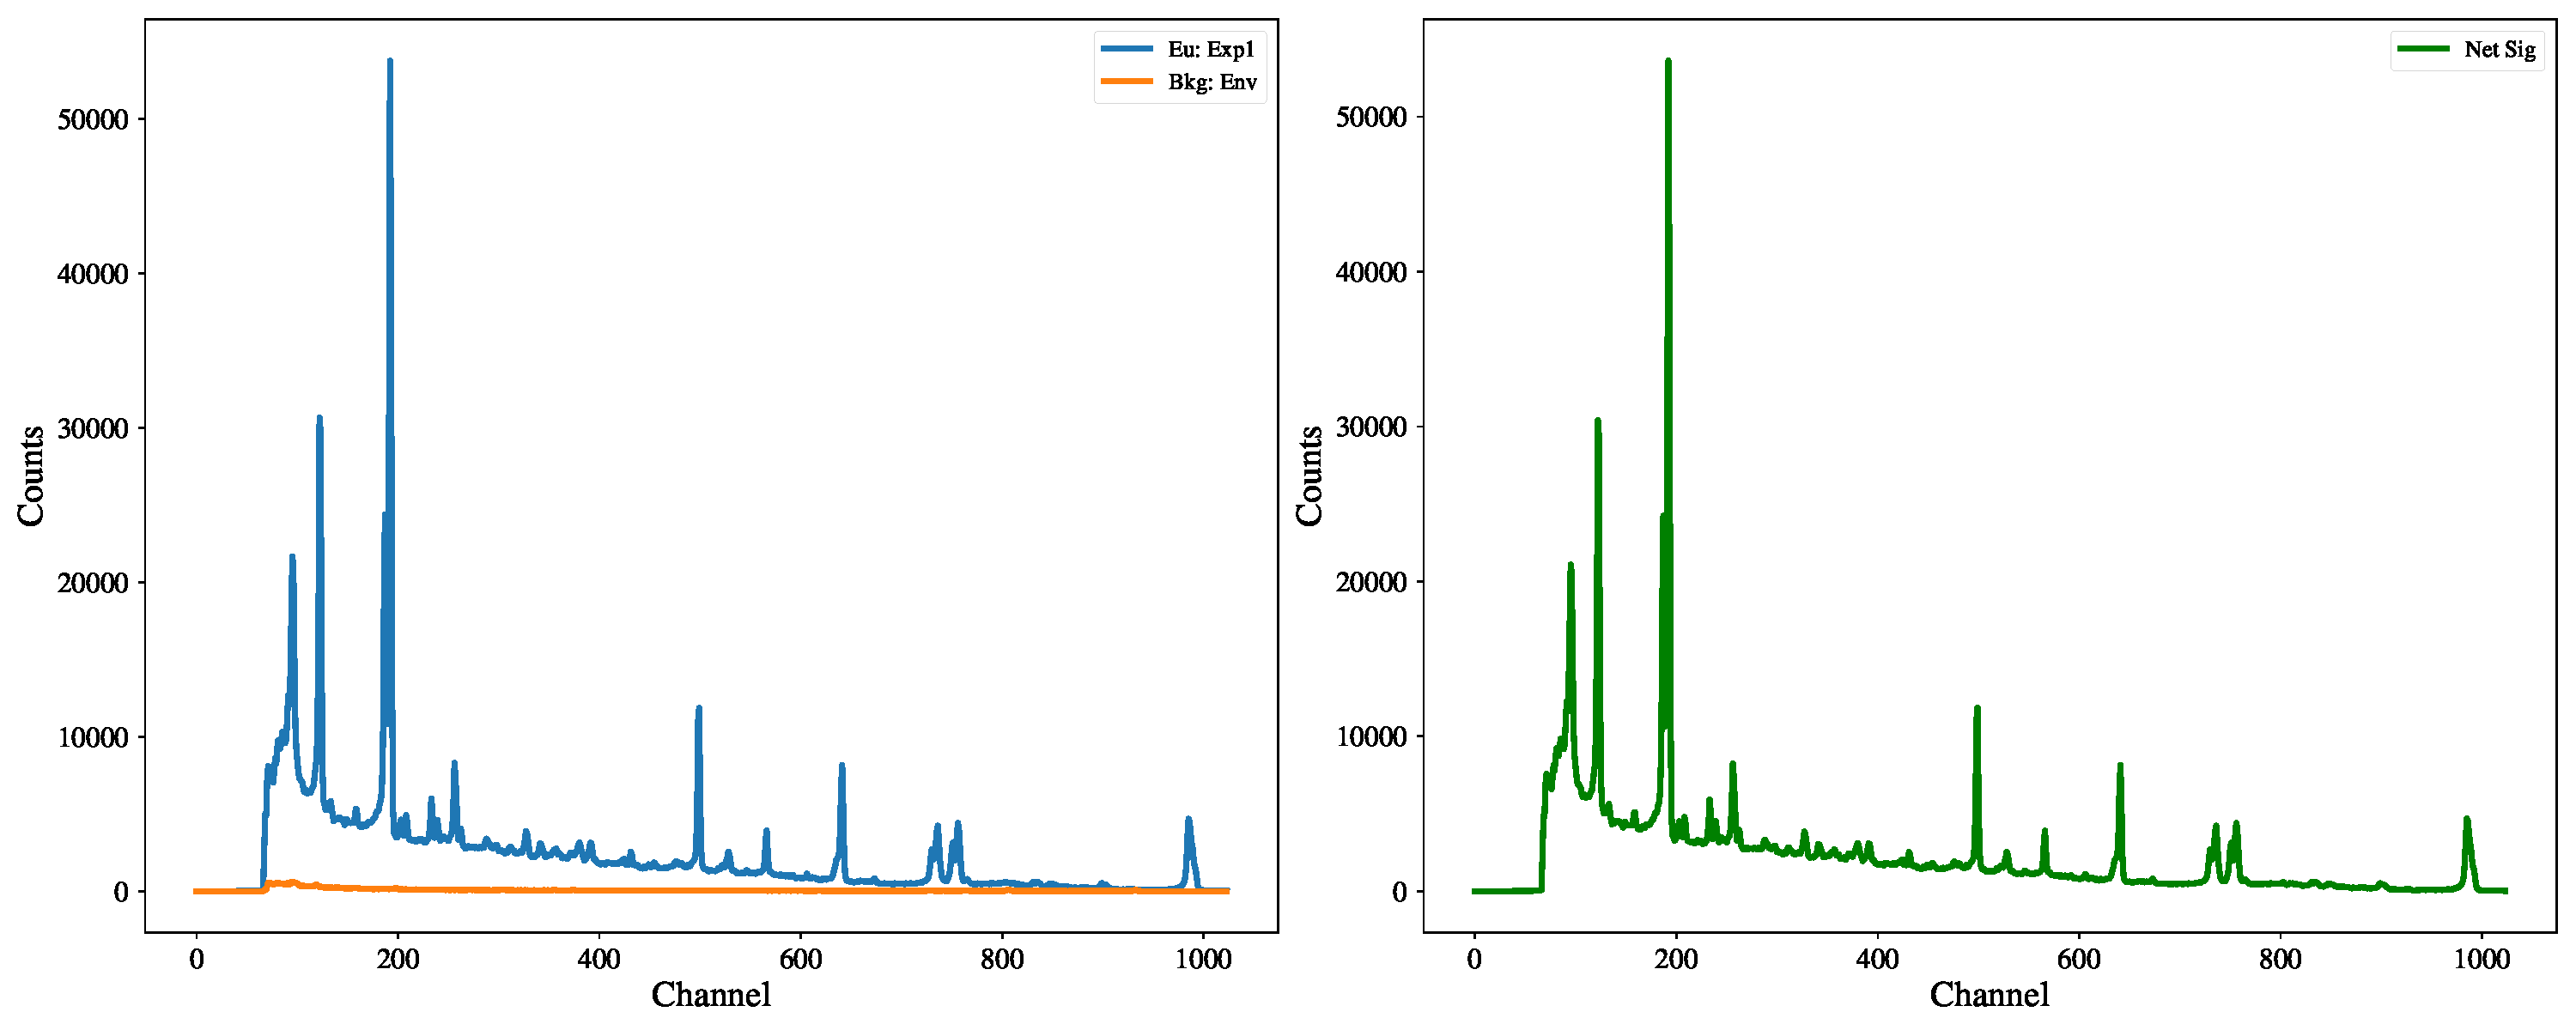
\includegraphics[width=\textwidth]{../plots/Eu_full_net.pdf}
    \caption{$^{152}\text{Eu}$第一次刻度的测量结果\label{fig:152Eu_Full}}
\end{figure}
如果利用上述$^{60}\text{Co}$进行刻度的结果对$^{152}\text{Eu}$进行粗测,结果如图\ref{fig:Roughly_Cali_full}。
\begin{figure}
    \centering
    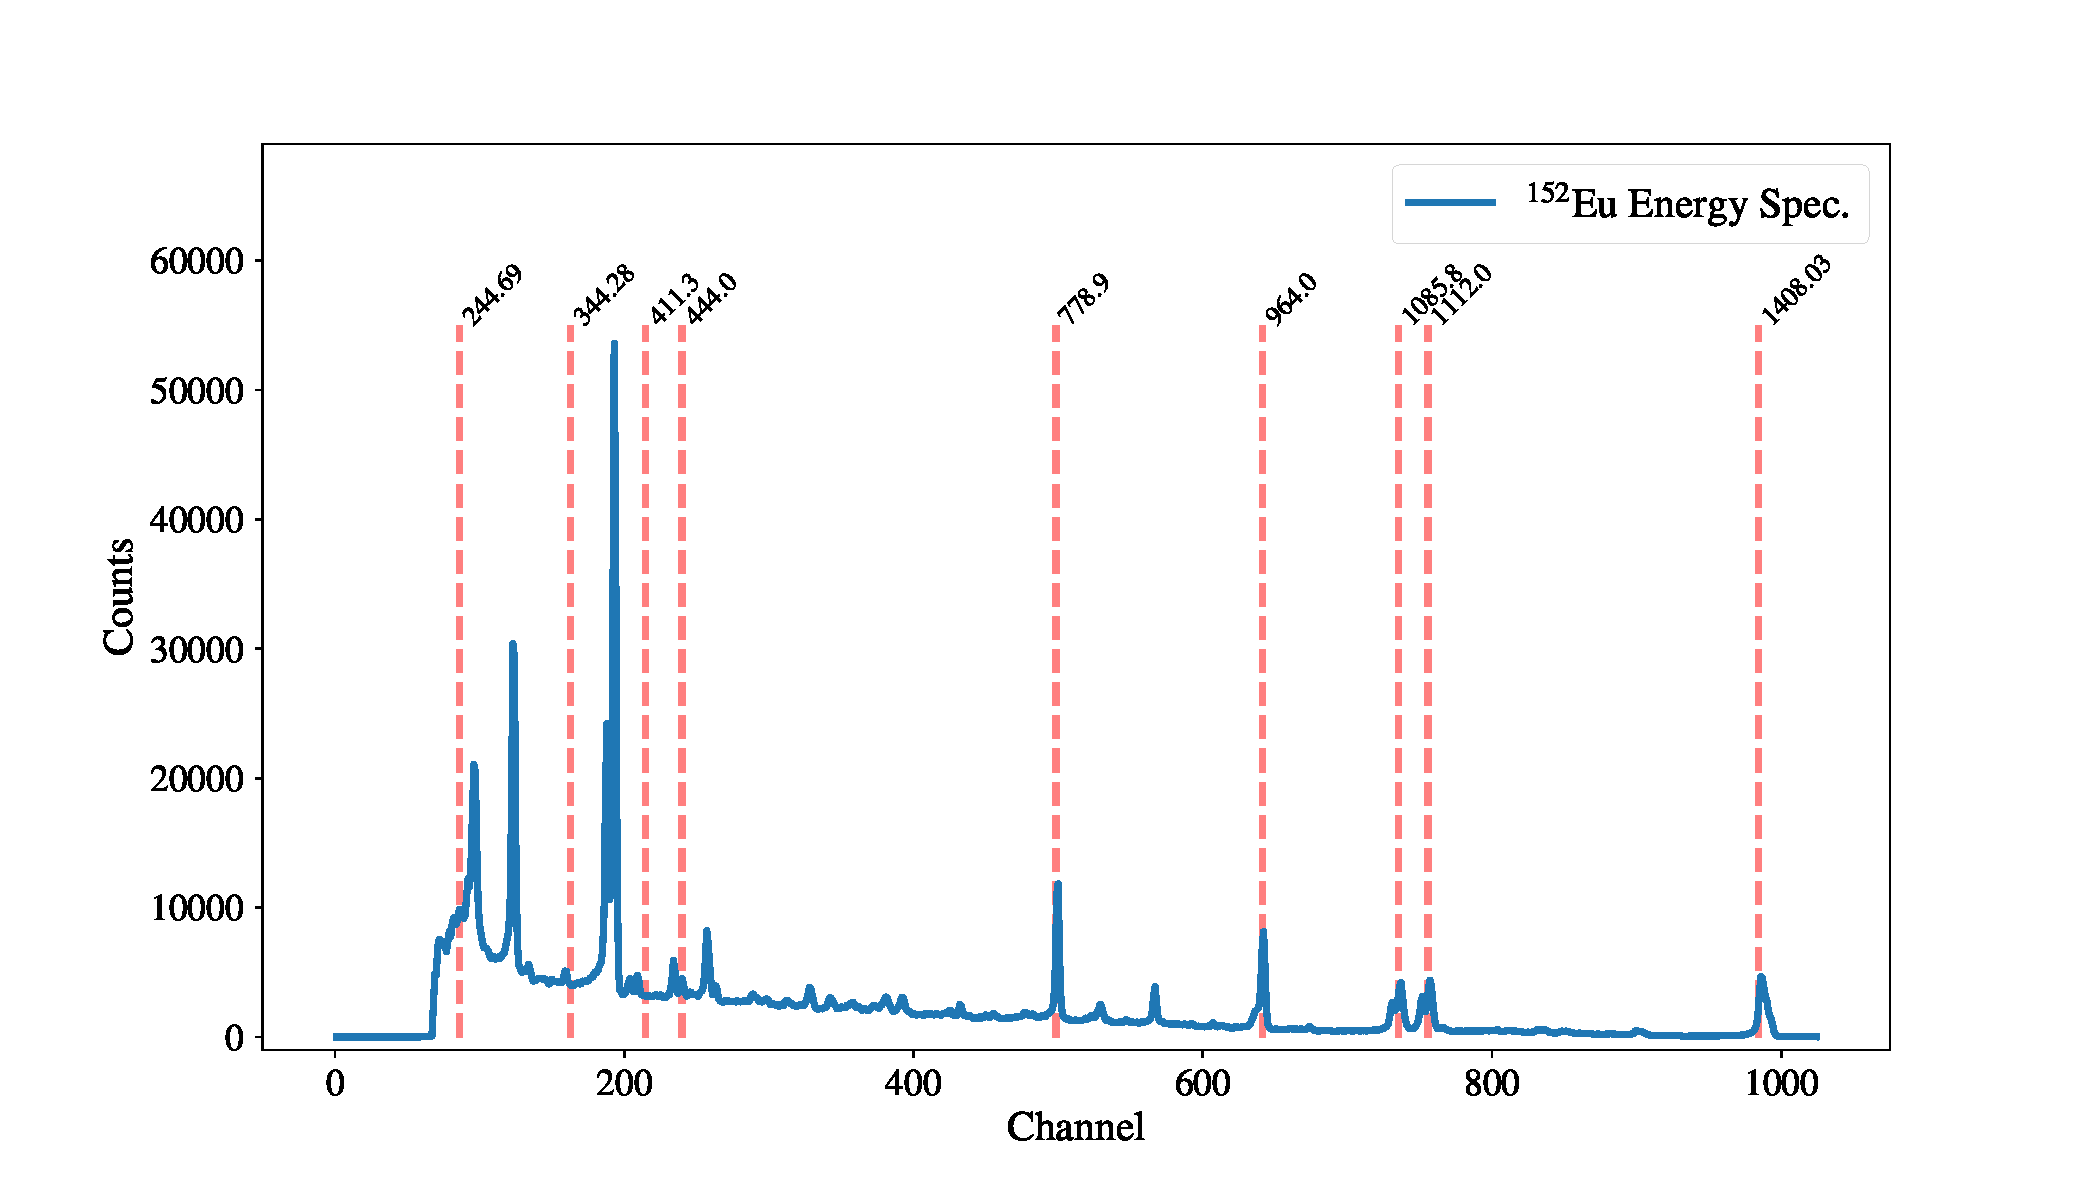
\includegraphics[width=\textwidth]{../plots/Roughly_Cali_full.pdf}
    \caption{利用$^{60}\text{Co}$的粗刻度结果对$^{152}\text{Eu}$的峰位进行预测,并和测量结果进行比较\label{fig:Roughly_Cali_full}}
\end{figure}
在高能区,粗测的刻度结果能够很好的解释实验观察到的峰位。但是能量较低的区间,则难以令人满意。因此,将低能区观测到的五个峰匹配上理论峰能量进行新的刻度,结果如下。

\section{致谢}
    感谢许金艳老师的实验指导,感谢刘寅绅同学和童星昱同学的讨论。也感谢张轩豪同学一起进行实验。
    \clearpage
    \appendix
    \appendixpage
    \section{思考题}
    \begin{enumerate}
        \item \begin{itemize}
            \item NaI(TI)探测:对$\gamma$射线,当能量大于$150\si{KeV}$时响应是线性的。其主要优点是密度大,原子序数高,对γ射线探测效率高。同时因为发光效率高,能量分辨率也较好。但必须密封使用以防止潮解。
            \item 高纯锗: 作为半导体探测器,必须用液态氮冷却条件下使用。他的优点一是空间分辨率好,分辨时间快;二是灵敏度高;三是在同样剂 量辐照下,输出的信号比电离室大。但也有能量响应差而不能做绝对测量和辐射损伤效应等缺点。
        \end{itemize}
        \item 相对效率曲线体现出不同能量下探测效率的相对大小。通过与已知活度的放射源比较可以将相对效率归一到绝对效率。
        在能量小于$2m_{e}$时,光子主要发生康普顿散射,能量会沉积在全能峰,所以探测效率随着能量增大逐渐增加。当能量大于$2m_{e}$时,开始发生电子对效应,高能量的电子和正电子可能在消耗完能量之前就从灵敏体积中逸出,在能谱中形成单逃逸峰或双逃逸峰,使全能峰的探测效率随能量增大而减小。
        \item 高纯锗探测器禁带宽度较窄($\sim 0.7\si{eV}$),需要低温真空(液氮冷却至$77\si{K}$左右)运
        行,保证锗晶体工作于半导体状态。同时,因为探测器十分灵敏,低温也可以防止电子因为温度自激发带来显著噪声。 
    \end{enumerate}
\end{document}